\chapter[Zeitabhängige Quellenverteilungen]{Felder zeitabhängiger Ladungs- und Stromverteilungen}

Nun suchen nach allgemeinen Lösungen der \textsc{Maxwell}-Gleichungen:

\begin{align*}
\div \vec{B}  \ &= \ 0 & \epsilon_0 \ \div\vec{E}  \ &= \ \rho\\
\rot\vec{E} \ + \ \dot{\vec{B}} \ &= \ 0 & \frac{1}{\mu_0}\rot\vec{B}\ - \ \epsilon_0\dot{\vec{E}}  \ &= \ \vec{j}
\end{align*}

\section{Viererpotential}

\ \\
Die Gleichung $\div \vec{B} = 0 $ wird erfüllt durch $\vec{B}=\rot\vec{A}$.\\
Die Gleichung $\rot\vec{E} \ + \ \dot{\vec{B}} = 0 \; \Rightarrow \; \rot (\vec{E} + \dot{\vec{A}}) =0$ wird erfüllt durch $\vec{E} + \dot{\vec{A}}= - \grad\varphi$\\
\ \\
\ \\
Somit können alle Felder durch das \textbf{Viererpotential} $(\varphi,\vec{A})$ ausgedrückt werden, sodass im Endeffekt immer 4 skalare Felder bestimmt werden müssen:

\begin{empheq}[box=\highlightbox]{align*}
\vec{B} \ &= \ \rot \vec{A}\vphantom{\big|}\\
\vec{E} \ &= \ - \grad \varphi - \dot{\vec{A}}
\end{empheq}

\newpage
Das Einsetzen in die \textsc{Maxwell}-Gleichungen und Ausnutzung des \textsc{d'Alembert}-Operators  $\Dalembert  =  \frac{1}{c^2}\pddiff{}{t} - \laplace$ liefert:

\begin{align*}
\div\vec{E}  \ &= \  \frac{\rho}{\epsilon_0} \qquad  & \rot \vec{B} \ - \ \epsilon_0\mu_0\vec{E}  \ = \ \mu_0\vec{j}\\
-\laplace\varphi \ - \ \div\dot{\vec{A}}  \ &= \ \frac{\rho}{\epsilon_0}	\qquad	& \rot\rot\vec{A} \ + \ \frac{1}{c^2}\grad\dot{\varphi} \ + \ \frac{1}{c^2} \ddot{\vec{A}}  \ = \ \mu_0\vec{j}\\
&& \nabla(\nabla\vec{A}) \ - \ \laplace\vec{A} \ + \ \frac{1}{c^2}\ddot{\vec{A}} \ + \ \frac{1}{c^2}\partial_t \ \nabla\varphi  \ = \ \mu_0\vec{j}\\
\ \\
\Dalembert\varphi  \ - \ \partial_t\left(\frac{1}{c^2}\partial_t\ \varphi \ + \ \nabla\vec{A}\right)  \ &= \ \frac{\rho}{\epsilon_0}  \qquad &
\Dalembert\vec{A} \ + \ \nabla\left(\frac{1}{c^2} \partial_t \ \varphi \ + \ \nabla\vec{A}\right) \ = \ \mu_0\vec{j}
\end{align*}

\ \\

Die Potentiale sind damit aber nicht eindeutig, sondern nur bis auf eine beliebige Eichung der Form $\vec{A}\rightarrow\vec{A}+\grad\chi$ und $\varphi \rightarrow\varphi-\partial_t\chi$ genau bestimmt. Eine \textbf{gleichwertige Umeichung} von $\vec{A}$ und $\varphi$ lässt die Felder unter solche einer Transformation invariant. Die Eichtransformation enthält genau eine skalare Funktion $\chi$, anders gesprochen eine skalare Bedingung. Für uns günstig ist die sogenannte \textbf{\textsc{Lorentz}-Eichung}, da sie die Felder invariant unter \textsc{Lorentz}-Transformation lässt und sie somit geeignet bleiben für relativistische Probleme. Die \textsc{Lorentz}-Transformation hat folgende Gestalt:

\begin{equation*}
\frac{1}{c^2} \ \pdiff{\varphi}{t} \ + \ \div \vec{A}  \ = \ 0
\end{equation*} 

Mit der \textsc{Lorentz-Eichung} erhält man als Gleichungen für die Potentiale:

\begin{equation*}
\Dalembert\varphi  \ = \ \frac{\rho}{\epsilon_0}	\qquad  \qquad		\Dalembert\vec{A}  \ = \ \mu_0\vec{j} 
\end{equation*}

Hieran lässt sich auch einfach überprüfen, dass man die Gleichungen für die statischen Probleme leicht aus denen mit Zeitabhängigkeit erhalten kann mittels $\partial_t \rightarrow 0; \ \Dalembert \rightarrow \laplace$:

\begin{equation*}
\laplace\varphi  \ = \ -\frac{\rho}{\epsilon_0} \quad\text{(s. Kap.3)} \qquad	\laplace\vec{A} \ = \ -\mu_0\vec{j} \quad\text{(s. Kap. 4)} 	
\end{equation*}

\newpage
\underline{\textbf{Wichtige Eichungen:}}

\begin{enumerate}

\item \textbf{\textsc{Lorentz}-Eichung}

\begin{equation*}
\frac{1}{c^2} \partial_t \ \varphi \ + \ \div\vec{A} \ = \ 0
\end{equation*}

Die \textsc{Lorentz}-Eichung fixiert die Potentiale nicht; eine Umeichung der Form $\Dalembert\chi=0$ ist immer noch möglich.

\item \textbf{\textsc{Coulomb}-Eichung}

\begin{align*}
\div\vec{A} \ = \ 0 \qquad\qquad \Rightarrow \qquad\qquad -\laplace\varphi \ &= \ \frac{\rho}{\epsilon_0}\\
\Dalembert\vec{A} \ &= \ \mu_0\vec{j} \  - \ \frac{1}{c^2}\ \frac{\partial^2 \ \varphi}{\partial t \partial \vec{r}} 
\end{align*}

Die \textsc{Coulomb}-Eichung ist hier dieselbe wie in der Elektrostatik plus entsprechende Korrekturen.

\item \textbf{Transversale Wellen}

\begin{align*}
\varphi \ = \ 0 \qquad\qquad\Rightarrow\qquad\qquad \frac{1}{c^2}\ddot{\vec{A}}\ + \ \rot\rot\vec{A} \ &= \ \mu_0\vec{j}\\
- \frac{\partial^2 \ \vec{A}}{\partial t \partial \vec{r}}  \ &= \ \frac{\rho}{\epsilon_0} 
\end{align*}
\end{enumerate}

\section{Retardierte Potentiale}

\ \\
Wir haben nun eine inhomogene, lineare Differentialgleichung der Form $\Dalembert u \ = \ \xi$ vorliegen, zu deren Lösung wir die \textsc{Green}'sche Funktion $G(\vec{r},\vec{r}',t,t')$ heranziehen, welche die DGL $\;\Dalembert G = 4\pi \delta(\vec{r}-\vec{r}')\delta(t-t')$ löst.\\
Da $G$ translationsinvariant sein soll, kann es nur von $\vec{r}-\vec{r}'$ und $t-t'$ abhängen. Weiterhin erhalten wir aus der Rotationssymmetrie des Problems, dass $G$ nur von $|\vec{r}-\vec{r}'|=:|\vec{R}|$ abhängen kann.
\newpage
Zur weiteren Lösung der DGL $\; \Dalembert G = 4\pi\delta(\vec{r}-\vec{r}')\delta(t-t')$ bilden wir nun ihre \textsc{Fourier}-Transformierte (s. Kap. 1):

\begin{align*}
\left(\pddiff{}{\vec{R}} \ - \ \frac{1}{c^2}(i\omega)^2\right)G\left(\vec{R},\omega\right)  \ &= \ 4\pi\delta(\vec{R})\;\Bigg | \; \frac{\omega}{c} \ = \ k; \text{ benutze Kugelkoord.}\\
\ddiff{}{R}G_k(R) \ + \ k^2 G_k(R) \ &= \ 4\pi\delta(R) \ \Bigg |\cdot R \neq 0\\
\ddiff{}{R}(R \ G_k) \ + \ k^2 \cdot (R \ G_k) \ &= \ 0 \quad\qquad\text{homogene DGL}\\
\ \\
\text{Lsg.: } R \ G_k(R) \ &= \ A\cdot e^{ikR} \ + \ A\cdot e^{-ikR}
\end{align*}

Die Inhomogenität $\delta(\vec{R})$ ist daher sehr wichtig nahe $\vec{R}=0$. Dort ist $k \cdot R \ll 1$, wodurch $k^2 \cdot R \ G_k$ vernachlässigbar wird gegenüber $\ddiff{}{R}(R\cdot G_k)$. Dann reduziert sich die DGL auf:

\begin{equation*}
\laplace_R G_k(R)  \ = \ - 4 \pi \delta(\vec{R})
\end{equation*}

Im Grenzwert $\lim\limits_{kR \rightarrow 0}{G_k(R)}  \ = \ \frac{1}{R}$ ist die allgemeine Lösung für $G$ also:

\begin{equation*}
G_k  \ = \ A \cdot G_k^+(R) \ + \ B\cdot G_k^- (R), \quad G_k^{\pm}  \ = \ \frac{e^{\pm i k R}}{R},\quad A+B=1
\end{equation*}

Nun können wir $G_k^{\pm}(R)$ rücktransformieren zu $G^{\pm}(\vec{R},\tau)$:

\begin{equation*}
G^{\pm}(\vec{R},\tau)  \ = \  \frac{1}{2\pi} \Int{-\infty}{\infty}{\omega} \frac{e^{-\pm i\omega\tau}}{R}\cdot e^{-i\omega\tau}  \ = \ \frac{1}{R}\delta\left(\tau\mp \frac{R}{c}\right) \qquad \left(\text{mit }k=\frac{\omega}{c}\right)
\end{equation*}

Bezogen auf unser Anfangsproblem entspräche diese Lösung:

\begin{equation*}
G^{\pm}(\vec{r},t,\vec{r}',t')  \ = \ \frac{\delta\left(t' \ - \ \left(t \mp \frac{|\vec{r}-\vec{r}'|}{c}\right)\right)}{|\vec{r}-\vec{r}'|}
\end{equation*}

Der Unterschied zwischen $G^+$ und $G^-$ liegt in den Randbedingungen in der Zeit. Anschaulich beschreibt $G$ die Reaktion des Systems bei $(\vec{r},t)$ aufgrund einer Störung (Inhomogenität) bei $(\vec{r}',t')$. Um die Kausalität nicht zu verletzen, muss demzufolge $G(t<t')=0$ gelten. Dies ist erfüllt für die \textbf{retardierte \textsc{Green}'sche Funktion} $G^+$, da hier die Wirkung \underline{nach} der Ursache auftritt und sich mit Lichtgeschwindigkeit ausbreitet (Verzögerung $\tau = \frac{R}{c}$). $G^-$ nennt man auch die \textbf{avancierte \textsc{Green}'sche Funktion}, aber aus naheliegenden Gründen wird sie hier nicht weiter behandelt.\\
Die (kausale) Lösung unserer inhomogenen DGL vom Anfang $\Dalembert u = \xi$ lautet damit:

\begin{equation*}
u(\vec{r},t) \ = \ \underbrace{u_0(\vec{r},t)}_{\text{homogene Lsg.}} \ + \ \frac{1}{4\pi}\int\d V' \d t' G^+(\vec{r},t,\vec{r}',t')\xi (\vec{r}',t')
\end{equation*}

Diese Lösung können wir nun auf unsere DGLn zur Bestimmung des Viererpotentials $\Dalembert\varphi = \frac{\rho}{\epsilon_0}$ und $\Dalembert\vec{A}= \mu_0\vec{j}$ anwenden:\\
Für eine räumlich begrenzte Quellenverteilung und der Randbedingung, dass die Felder im Unendlichen gegen Null gehen, erhalten wir, wenn wir als homogene Lösungen $\varphi_0=0$ und $\vec{A}_0=0$ setzen, folgende allgemeine Lösung der \textsc{Maxwell}-Gleichungen:

\begin{empheq}[box=\highlightbox]{align*}
\varphi(\vec{r},t)  \ &= \ \frac{1}{4\pi\epsilon_0} \ \Int{}{\vphantom{\big|}}{V'} \ \frac{\rho\left(\vec{r'}, t \ - \ \frac{|\vec{r}-\vec{r}'|}{c}\right)}{|\vec{r}-\vec{r}'|}\\
\ \\
\vec{A}(\vec{r},t)  \ &= \ \ \frac{\mu_0}{4\pi} \ \ \Int{\vphantom{A}}{}{V'} \ \frac{\vec{j}\left(\vec{r}',t \ - \ \frac{|\vec{r}-\vec{r}'|}{c}\right)}{|\vec{r}-\vec{r}'|} 
\end{empheq}

Die obigen Gleichungen beschreiben \textbf{retardierte Potentiale}, welche folgendermaßen interpretiert werden können:\\
$\rho$ und $\vec{j}$ sind die Ursachen für die Wirkungen $\varphi$ und $\vec{A}$, welche allerdings eine Laufzeitverzögerung von $\frac{|\vec{r}-\vec{r}'|}{c}$ aufweisen.\\
\ \\

Die Überprüfung der gefundenen Lösung erfolgt leicht durch Einsetzen in $ \ \Dalembert\varphi=\frac{\rho}{\epsilon_0}$ und $\ \Dalembert\vec{A} = \mu_0\vec{j}$. Setzt man sie außerdem in die \textsc{Lorentz}-Eichung $\frac{1}{c^2}\partial_t \ \varphi + \div\vec{A} =0$ ein, so führt dieses auf die Kontinuitätsgleichung $\dot{\rho} + \div\vec{j}=0$.\\
\ \\
\underline{Bemerkung:}\\
Auch die avancierte \textsc{Green}-Funktion $G^-$ erfüllt die inhomogenen Wellengleichungen $\ \Dalembert\varphi=\frac{\rho}{\epsilon_0}$ und $\ \Dalembert\vec{A} = \mu_0\vec{j}$. Dies liegt mathematisch daran, dass die Wellengleichungen $c$ quadratisch enthalten, das Potential aber nur linear. Da diese Lösung aber akausal ist und nur $G^+$ die Kausalität erhält, zeichnet ebenjene Wahl von $G^+$ die Richtung der Zeit aus.


\section{\textsc{Hertz}'scher Dipol}

Wir betrachten nun als konkretes Beispiel für eine zeitabhängige Quellenverteilung einen oszillierenden Dipol: zwei Ladungen $\pm Q$ befinden sich entlang einer Achse in variablen Abstand $\vec{a}(t)$ voneinander entfernt. Somit gilt für die Stromdichte $\vec{j} := \vec{J}\cdot\delta(\vec{r})$, dass $\vec{j}=\dot{\vec{a}}\cdot Q \cdot\delta(\vec{r}-\vec{r}_a)$ ist. Im Dipollimit $\vec{a}\rightarrow 0$ folgt somit $\vec{j}=\dot{\vec{p}}\cdot\delta(\vec{r})$.\\
Allgemein gilt somit: $\vec{J}(t) = \Int{}{}{V} \vec{j}(\vec{r},t) = \dot{\vec{p}}$, oder genauer:

\begin{align*}
\dot{\vec{p}} \ = \ &\Int{}{}{V}\vec{r}\dot{\rho} \ = \ -\Int{}{}{V}\vec{r}\div\vec{j} \ = \ \Int{}{}{V}\left(\vec{j}\cdot\nabla\right)\cdot\vec{r} \ + \ \underbrace{\text{Oberflächenintegral}}_{\rightarrow 0} \\
\overset{\nabla\circ\vec{r}=\mathbbm{1}}{=} \ &\Int{}{}{V}\vec{j}  \ = \ \vec{J}
\end{align*}

Nun wollen wir die  (abgestrahlten) Felder des oszillierenden Dipols berechnen, wozu wir zunächst die retardierten Potentiale aufstellen:

\begin{equation*}
\vec{A}(\vec{r},t) \ = \ \frac{\mu_0}{4\pi}\ \Int{}{}{V'} \ \frac{\delta(\vec{r})\vec{J}\left(t \ - \ \frac{|\vec{r}-\vec{r}'|}{c}\right)}{|\vec{r}-\vec{r}'|} \ = \ \frac{\mu_0}{4\pi}\ \frac{\dot{\vec{p}}\left(t\ - \ \frac{r}{c}\right)}{r}
\end{equation*}

$\varphi$ erhalten wir aus der Ladungsverteilung zu $\vec{j}$ und aus der \textsc{Lorentz}-Eichung:

\begin{equation*}
\varphi(\vec{r},t)  \ = \ -\frac{1}{4\pi\epsilon_0} \ \frac{\vec{r}}{r} \ \pdiff{}{r} \ \frac{\vec{p}\left(t\ - \ \frac{r}{c}\right)}{r} \ + \ \text{zeitunabhängiges Potential}
\end{equation*}

Jetzt können die Felder $\vec{B}=\rot\vec{A}$ und $\vec{E}=-\grad\varphi-\dot{\vec{A}}$ berechnet werden.\\
$\left(\text{Notationshinweis: }\vec{p}|_{\text{ret}} \text{ steht für }\vec{p}\left(t-\frac{r}{c}\right)\right):$\\

\begin{align*}
\vec{B} \ &= \ \frac{\vec{r}}{r}\times\pdiff{\vec{A}}{r} \ = \ - \frac{\mu_0}{4\pi} \ \frac{\vec{r}}{r}\times \left(\frac{\ddot{\vec{p}}}{c}\ + \ \frac{\dot{\vec{p}}}{r}\right)_{\text{ret}}\\
\ \\
\vec{E} \ &= \ - \grad\varphi - \dot{\vec{A}} \ = \ -\grad\left(\frac{1}{4\pi\epsilon_0} \ \frac{\vec{r}}{r} \left[\frac{\vec{p}}{r^2} \ + \ \frac{\dot{\vec{p}}}{cr}\right]_{\text{ret}}\right) \ - \ \dot{\vec{A}}\\
\ \\
&= \ -\frac{1}{4\pi\epsilon_0 \cdot r} \left(\frac{\ddot{\vec{p}}}{c^2} \ - \ \frac{\left(\ddot{\vec{p}}\cdot\vec{r}\right)\vec{r}}{c^2 \ r^2} \ + \ \frac{\dot{\vec{p}}}{c \ r} \ - \ 3 \frac{\left(\dot{\vec{p}}\cdot\vec{r}\right)\vec{r}}{c \ r^3} \ + \ \frac{\vec{p}}{r^2} \ - \ 3 \frac{\left(\vec{p}\cdot\vec{r}\right)\vec{r}}{r^4}\right)_{\text{ret}}
\end{align*}

\newpage
\underline{Spezialfälle:}
\begin{enumerate}
\item \textbf{statischer Dipol} \qquad $\partial_t  \ = \ 0$

\begin{align*}
\Rightarrow \qquad \vec{B}  \ &= \ 0\\
\vec{E} \ &= \ - \frac{1}{4\pi\epsilon_0 \ r^3}\left(\vec{p} \ - \ \frac{3(\vec{p}\cdot\vec{r})\cdot\vec{r}}{r^2}\right)
\end{align*}

\item \textbf{harmonische Schwingung} \qquad $\vec{p} \ \sim \ e^{-i\omega t}$

\begin{align*}
\Rightarrow \qquad \partial_t \ &\rightarrow \ -i\omega\\
\frac{1}{c}\partial_t \ &\rightarrow \ - \frac{i\omega}{c}  \ = \ -i \frac{2\pi}{\lambda}  \ = \ -ik
\end{align*}

Für den Fall der harmonischen Schwingung von $\vec{p}$ wollen wir nun die Abstandsabhängigkeit der Feldbeiträge betrachten. Dazu sortieren wir die Beiträge nach ihren Ordnungen $\sigma(.)$:

\begin{align*}
\vec{B} \ &\sim \ - \frac{\mu_0 \vec{r}}{4\pi \ r^2} \times \Bigg(\underbrace{\sigma\left(\frac{\dot{\vec{p}}}{\lambda}\right)}_{\text{Fernfeld}} \; + \; \underbrace{\sigma\left(\frac{\dot{\vec{p}}}{r}\right)}_{\text{Nahfeld}}\Bigg)\\
\vec{E} \ &\sim \ - \frac{1}{4\pi\epsilon_0} \cdot \left(\sigma\left(\frac{\vec{p}}{\lambda^2}\right) \; + \; \sigma\left(\frac{\vec{p}}{r \cdot \lambda}\right) \; + \; \sigma\left(\frac{\vec{p}}{r^2}\right)\right)
\end{align*}

\ \\
\textbf{Nahfeld:} $\quad r \ll \lambda$

\begin{empheq}[box=\highlightbox]{align*}
\vec{B}(\vec{r},t)  \ &= \ \frac{\mu_0\vphantom{\big|}}{4\pi\ r^2} \ \left(\dot{\vec{p}} \times \frac{\vec{r}}{r}\right)_{\text{ret}}\\
\vec{E}(\vec{r},t)  \ &= \ \frac{1}{4\pi\epsilon_0 \ r^2\vphantom{\big|}} \ \left(\frac{3(\vec{p}\cdot\vec{r})\vec{r}}{r^2} \ - \ \vec{p}\right)_{\text{ret}} 
\end{empheq}

Für das Nahfeld verzichtet man häufig auf die Retardierung, da sie kaum ins Gewicht fällt:

\begin{equation*}
\vec{p} \ \sim \ e^{-i\omega\left(t-\frac{r}{c}\right)}  \ = \ e^{-i\omega t} \cdot \underbrace{\; e^{2\pi i \frac{r}{\lambda}}\;}_{1+2\pi i \frac{r}{\lambda}+\ldots \approx 1}
\end{equation*}

\ \\
\textbf{Fernfeld:} $\quad r \gg \lambda \qquad\left(\frac{\vec{r}}{r} \ = \ \vec{e}_r\right)$

\begin{empheq}[box=\highlightbox]{align*}	
\vec{B}(\vec{r},t)  \ &= \ \frac{\mu_0\vphantom{\big|}}{4\pi \ r \ c} \left(\ddot{\vec{p}}\times\vec{e}_r\right)_{\text{ret}}\\
\vec{E}(\vec{r},t)  \ &= \ \frac{\mu_0}{4\pi \ r\vphantom{\big|}} \left(\left(\ddot{\vec{p}}\cdot\vec{e}_r\right)\cdot\vec{e}_r \ - \ \ddot{\vec{p}}\right)_{\text{ret}}  \ = \ \frac{\mu_0}{4\pi \ r}\left(\ddot{\vec{p}}\times\vec{e}_r\right)_{\text{ret}}\times\vec{e}_r  \ = \ c\cdot\vec{B}\times\vec{e}_r
\end{empheq}

Bei harmonisch schwingendem $\vec{p}$ breiten sich $\vec{E}$ und $\vec{B}$ also radial als transversale Welle aus:

\begin{equation*}
e^{-i\omega\left(t-\frac{r}{c}\right)}  \ = \ e^{i(kr-\omega t)} \qquad \text{mit } k  \ = \  \frac{\omega}{c}
\end{equation*}

Dabei fallen $|\vec{E}|$ und $|\vec{B}|$ nur mit $\frac{1}{r}$ ab!
\end{enumerate}


\section{Energieabstrahlung des \textsc{Hertz}'schen Dipols}

\textbf{Energiedichte:}

\begin{equation*}
w  \ = \ \frac{\epsilon_0}{2} \vec{E}^2  \ +  \ \frac{1}{2\mu_0} \vec{B}^2  \ = \ \frac{\vec{B^2}}{\mu_0}
\end{equation*}

\ \\
\textbf{Energiestromdichte:}

\begin{align*}
\vec{S}_P  \ &= \ \frac{1}{\mu_0} (\vec{E}\times\vec{B})  \ = \ \frac{c}{\mu_0} (\vec{B}\times\vec{e}_r\times\vec{B})  \ = \  \frac{c}{\mu_0}\Big(\vec{e}_r\vec{B}^2 \ - \ \vec{B}(\underbrace{\vec{n}\cdot\vec{B}}_{=0})\Big)  \ = \ c\cdot\vec{e}_r\cdot w\\
\alignedbox{\hspace{.5em}|\vec{S}_P|  \ }{= \ \frac{\mu_0}{(4\pi)^2c}\cdot \frac{\left(\ddot{\vec{p}}\times\vec{e}_r\right)^2}{r^2} \ = \ \frac{\mu_0}{(4\pi)^2c}\cdot\frac{\ddot{\vec{p}}^2\sin^2\theta}{r^2} \hspace{.5em}} \qquad \left(\text{mit } \theta = \sphericalangle(\ddot{\vec{p}},\vec{e}_r)\right)
\end{align*}

Man sieht hieran leicht, dass senkrecht zur Dipolachse $\vec{a}$ am stärksten ausgestrahlt wird (da auch $\ddot{\vec{p}}\perp \vec{a}$).

\ \\
\textbf{Frequenzabhängigkeit der abgestrahlten Leistung:}

\begin{equation*}
|\vec{S}_P|  \ \sim \ |\ddot{\vec{p}}|^2 \ \sim p^2 \ \omega^4
\end{equation*}

Diese Frequenzabhängigkeit ist charakteristisch für Dipolstrahlung.

\newpage
\textbf{Abgestrahlte Leistung:}

\begin{align*}
N  \ &= \ \Iint{}{}{\vec{A}_F} \cdot \vec{S}_P  \ = \ \Int{}{}{\Omega}r^2 \ \frac{\mu_0}{(4\pi)^2c}\cdot\frac{\ddot{\vec{p}}^2\sin^2\theta}{r^2}  \ = \ \frac{\mu_0\ddot{\vec{p}}^2}{(4\pi)^2c} \ \Int{}{}{\Omega}\sin^2\theta\\
&= \ \frac{\mu_0\ddot{\vec{p}}^2}{(4\pi)^2c} \Int{0}{2\pi}{\phi}\Int{-1}{1}{(\cos\theta)} \ (1 \ - \ \cos^2\theta) \ = \ \frac{\mu_0\ddot{\vec{p}}^2}{(4\pi)^2c} \cdot 2\pi \cdot \left(2-\frac{2}{3}\right) \ = \ \frac{2}{3} \ \frac{\mu_0}{4\pi c} \ddot{\vec{p}}^2_{\text{ret}}
\end{align*}

Wenn wir einen harmonisch oszillierenden Dipol betrachten, so gilt für $\ddot{\vec{p}}$:

\begin{align*}
\vec{p}  \ &= \ \vec{p}_0 \cos\omega t \qquad \Rightarrow \qquad \ddot{\vec{p}}^2  \ = \ \omega^4\vec{p}_0^2\cos^2\omega t\\
\Rightarrow \langle\ddot{\vec{p}}^2\rangle_T  \ &= \  \omega^4\vec{p}_0^2 \langle\cos^2\omega t\rangle_T  \ = \ \frac{1}{2} \omega^4 \vec{p}_0^2
\end{align*}

Damit gilt also für die (über eine Periode gemittelte) abgestrahlte Leistung:

\begin{empheq}[box=\highlightbox]{equation*}
\langle N \rangle_T  \ = \  \frac{\mu_0 \ \omega^4\ \vec{p}_0^2\vphantom{\big|}}{12\pi \ c\vphantom{\big|}}
\end{empheq}

\section[Strahlung räumlich begrenzter Quellen]{Strahlungsfeld einer räumlich begrenzten Quellenverteilung}

Wir betrachten nun eine beliebige Quellenverteilung am Ort $\vec{r}'$ mit der maximalen räumlichen Ausdehnung $a$. Es gilt ganz allgemein für das Vektorpotential am Ort $\vec{r}$:

\begin{equation*}
\vec{A}(\vec{r},t) \ = \ \frac{\mu_0}{4\pi}\Int{}{}{V'} \ \frac{\vec{j}\left(\vec{r}',t\ - \ \frac{|\vec{r}-\vec{r}'|}{c}\right)}{|\vec{r}-\vec{r}'|}
\end{equation*}

Wir entwickeln nun den Ausdruck $\frac{1}{|\vec{r}-\vec{r}'|}$ für das Fernfeld $(r\gg a, |\vec{r}| \gg |\vec{r}'|)$:

\begin{align*}
\frac{1}{|\vec{r}-\vec{r}|}  \ &= \ \frac{1}{r} \ + \ \frac{\vec{r}\cdot\vec{r}'}{r^3} \ + \ \ldots \ \approx \ \frac{1}{r} \quad \text{(Dipolnäherung)}\\
|\vec{r}-\vec{r}'|  \ &= \ r \ - \ \frac{\vec{r}\cdot\vec{r}'}{r} \ + \ \ldots \ \approx \ r \ - \ \vec{e}_r \cdot \vec{r}'\\
\Rightarrow \quad \vec{A}(\vec{r},t)  \ &= \ \frac{\mu_0}{4\pi \ r} \underbrace{\Int{}{}{V'} \vec{j} \left(\vec{r}',t \ - \ \frac{r}{c} \ + \ \frac{\vec{e}_r\cdot\vec{r}'}{c}\right)}_{\equiv \dot{\vec{q}}\left(t \ - \ \frac{r}{c},\vec{e}_r\right)}
\end{align*}

Zum Vergleich: Das Vektorpotential für einen \textsc{Hertz}'schen Dipol ergab:

\begin{equation*}
\vec{A}  \ = \ \frac{\mu_0}{4\pi \ r} \ \dot{\vec{p}}\left(t \ - \ \frac{r}{c}\right)
\end{equation*}

Das $\vec{B}$-Feld erhalten wir aus dem eben gewonnenen Ausdruck für $\vec{A}$ durch $\vec{B}=\rot\vec{A}$:

\begin{align*}
\pdiff{}{\vec{r}}\left[\frac{1}{r} f \left(t-\frac{r}{c},\vec{e}_r\right)\right] \ &= \ \Bigg[\underbrace{-\frac{\vec{e}_r}{c}\partial_t}_{\sigma\left(\frac{1}{\lambda}\right)} \ - \ \underbrace{\frac{\vec{e}_r}{r}}_{\sigma\left(\frac{1}{r}\right)} \ + \ \underbrace{\pdiff{}{\vec{r}}\left(\vec{e}_r\cdot\pdiff{}{\vec{e}_r}\right)}_{\sigma\left(\frac{1}{r}\right)}\Bigg ] \left(\frac{1}{r}f\right) \ \approx \ - \frac{\vec{e}_r}{c} \partial_t \left(\frac{1}{r}f\right)\\
\ \\
\overset{r\gg\lambda}{\Rightarrow} \qquad\quad \alignedbox{\hspace{.5em}\vec{B}  \ }{= \ -\frac{\vec{e}_r}{c}\times\dot{\vec{A}}  \ = \  \frac{\mu_0}{4\pi \ c} \cdot \frac{\ddot{\vec{q}}\times\vec{e}_r}{r}\hspace{.5em}}
\end{align*}

Das $\vec{E}$-Feld erhalten wir aus der inhomogenen \textsc{Maxwell}-Gleichung: $\frac{1}{\mu_0}\rot\vec{B}= \vec{j} + \epsilon_0\dot{\vec{E}}$. Unter Beachtung, dass $\vec{j}=0$ außerhalb der Quellenverteilung ist, erhalten wir zunächst für $\dot{\vec{E}}$:

\begin{align*}
\dot{\vec{E}}  \ &= \ c^2 \ \rot\vec{B} \ \approx \ - \frac{\vec{e}_r}{c}\partial_t\times c^2 \vec{B}\\
\Rightarrow\qquad\quad \alignedbox{\hspace{.5em}\vec{E} \ }{= \ c\vec{B}\times\vec{e}_r  \ = \ \frac{\mu_0}{4\pi} \cdot \frac{\left(\ddot{\vec{q}}\times\vec{e}_r\right)\times\vec{e}_r}{r} \hspace{.5em}}
\end{align*}

Wir erhalten also wieder eine transversale Welle der Felder $\vec{E}$ und $\vec{B}$, welche beide mit $\frac{1}{r}$ abfallen. (Korrekturen aus höheren Termen fallen dabei schneller ab.)\\
Für die Energiestromdichte gilt damit:

\begin{equation*}
\vec{S}_P \ = \ \frac{1}{\mu_0} (\vec{E}\times\vec{B})  \ = \  \vec{e}_r \ \frac{\mu_0}{(4\pi)^2 c} \ \frac{\left(\ddot{\vec{q}}\times\vec{e}_r\right)^2}{r^2}
\end{equation*}

Der direkte Vergleich zwischen dem Fernfeld des \textsc{Hertz}'schen Dipols und dem Strahlungsfeld einer beliebigen Ladungsverteilung zeigt uns, dass mit $\dot{\vec{p}}\leftrightarrow\dot{\vec{q}}$ alle Fernfeldformeln identisch sind:

\begin{align*}
&\text{\textsc{Hertz}'scher Dipol:} \qquad\qquad\qquad\ \; \text{allgemein:}&\\
&\dot{\vec{p}}_{\text{ret}}  \ = \ \Int{}{}{V'} \vec{j}\left(\vec{r}',t-\frac{r}{c}\right) \qquad \qquad \dot{\vec{q}}  \ = \ \Int{}{}{V'}\vec{j}\left(\vec{r}',t-\frac{r}{c}+\frac{\vec{e}_r\cdot\vec{r}'}{c}\right)
\end{align*}

Den Ausdruck $\frac{\vec{e}_r\cdot\vec{r}'}{c}$ in $\dot{\vec{q}}$ kann man als die Laufzeit innerhalb der Quellen verstehen.


\section{Multipolentwicklung des Fernfelds}

Im vorigen Kapitel haben wir das Strahlungsfeld einer räumlich begrenzten Quellenverteilung mit beliebiger Zeitabhängigkeit betrachtet. Jetzt setzen wir uns mit dem Spezialfall auseinander, dass $\vec{j}\sim e^{-i\omega t}$ gilt:

\begin{equation*}
\vec{j}\left(t-\frac{r}{c} + \frac{\vec{e}_r \cdot\vec{r}'}{c}\right) \ \sim \ e^{-i\omega\left(t-\frac{r}{c}\right)} \ e^{-i\frac{\omega}{c} \vec{e}_r\cdot\vec{r}'}
\end{equation*}\\
\ \\

Wir entwickeln diesen Ausdruck für das Fernfeld $(r\gg a, r \gg \lambda)$ mit der zusätzlichen Annahme, dass es sich um eine "kleine Quelle" handelt $(\lambda\gg a)$:

\begin{align*}
&\frac{\omega}{c} \vec{e}_r \cdot \vec{r} \sim \frac{\omega}{c}a' \ = \  \frac{2\pi a}{\lambda} \ll 1 \quad\text{(Laufzeit in Quelle $\ll$ Periodendauer)}\\
\Rightarrow\quad &\vec{j}\left(t-\frac{r}{c}+\frac{\vec{e}_r\cdot\vec{r}'}{c}\right) \ \approx \ \vec{j}\left(t-\frac{r}{c}\right) \ + \ \frac{\vec{e}_r\cdot\vec{r}'}{c}\partial_t\vec{j}\left(t-\frac{r}{c}\right) \ + \ \ldots\\
&\dot{\vec{q}}  \ = \ \underbrace{\Int{}{}{V'}\vec{j}\left(\vec{r}',t-\frac{r}{c}\right)}_{=\dot{\vec{p}}_{\text{ret}}} \ + \ \frac{1}{c} \ \partial_t \Int{}{}{V'}\left(\vec{e}_r\cdot\vec{r}'\right) \ \vec{j} \left(\vec{r}', t- \frac{r}{c}\right) \ + \ \ldots
\end{align*}

Umformen ergibt:

\begin{align*}
\Int{}{}{V'} \left(\vec{e}_r\cdot\vec{r}'\right) \ \vec{j}  \ &= \ \frac{1}{2}\Int{}{}{V'} \left[\left(\vec{e}_r\cdot\vec{r}'\right)\vec{j} \ - \ \left(\vec{e}_r \cdot \vec{j}\right)\vec{r}'\right] \ + \ \Int{}{}{V'} \left[\left(\vec{e}_r\cdot\vec{r}'\right)\vec{j} \ + \ \left(\vec{e}_r\cdot\vec{j}\right)\vec{r}'\right]\\
&= \ -\vec{e}_r \times\underbrace{\frac{1}{2}\Int{}{}{V'}\left(\vec{r}'\times\vec{j}\right)}_{=\vec{m}} \ + \ \frac{\vec{e}_r}{2} \ \frac{1}{3} \dot{\tens{D}}'
\end{align*}

Denn:

\begin{align*}
\dot{\tens{D}} \ &= \ \Int{}{}{V}\underbrace{\dot{\rho}}_{-\nabla\vec{j}} \left(3\vec{r}\circ\vec{r} \ - \ \mathbbm{1} \vec{r}^2\right)  \ \overset{\text{part. Int.}}{=} \ \Int{}{}{V} \left(\vec{j}\cdot\nabla\right) \ \left(3\vec{r}\circ\vec{r} \ - \ \mathbbm{1}\vec{r}^2\right)\\
&= \ \Int{}{}{V}\left(3\vec{j}\circ\vec{r} \ + \ 3\vec{r}\circ\vec{j} \ - \ 2 \cdot \mathbbm{1} \ \left(\vec{j}\cdot\vec{r}\right)\right) \qquad\qquad(*)
\end{align*}

\newpage
Wir definieren:
\begin{align*}
\tens{D}'  \ &= \ \tens{D} \ + \ \mathbbm{1}\frac{\operatorname{Spur} \tens{D}}{3}  \ = \  \Int{}{}{V}\rho \ 3 \vec{r}\circ\vec{r}\\
\dot{\tens{D}} \ &= \ \Int{}{}{V}\left(3\vec{j}\circ\vec{r} \ + \ 3 \vec{r}\circ\vec{j}\right)
\end{align*}

Somit gilt für die Komponenten von $(*)$:\\

\begin{align*}
\left[\left(\vec{j}\cdot\nabla\right) \ \left(3\vec{r}\circ\vec{r} \ - \ \mathbbm{1} \vec{r}^2\right)\right]_{ij}  \ &= \ j_k \partial_k\ \left(3 r_i r_j \ - \ \delta_{ij} r_l r_l\right)\\
&= \ j_k \left(3\delta_{ij}r_j \ + \ 3r_i\delta_{jk} \ - \ \delta_{ij} 2 r_l \delta_{lk}\right)\\
&= \ 3j_i r_j \ + \ 3 r_i j_j \ - \ \delta_{ij} 2 j_k r_k
\end{align*}

Nun brauchen wir noch:\\

\begin{equation*}
\big[\left(\vec{m}\times\vec{e}_r\right)\times\vec{e}_r\big]\times\vec{e}_r  \ = \ \big[\vec{e}_r(\vec{m}\cdot\vec{e}_r) \ - \ \vec{m}(\underbrace{\vec{e_r}\cdot\vec{e}_r}_{=1})\big] \times \vec{e}_r \ = \ - \vec{m}\times\vec{e}_r
\end{equation*}\\

Und:\\
\begin{equation*}
\vec{e_r}\cdot\tens{D}'\times\vec{e}_r  \ = \ \vec{e}_r \cdot\tens{D}'\times\vec{e}_r \ + \ \underbrace{\vec{e}_r \ \mathbbm{1} \times\vec{e}_r}_{=\vec{e}_r\times\vec{r}_r =0} \ \frac{\operatorname{Spur}\tens{D}'}{3}  \ = \ \vec{e}_r\cdot\tens{D}\times\vec{e}_r
\end{equation*}

\begin{equation*}
\dot{\vec{q}}  \ = \  \left(\dot{\vec{p}} \ + \ \dot{\vec{m}} \times\frac{\vec{e}_r}{c} \ + \frac{\vec{e}_r}{6c}\cdot \ddot{\tens{
D}}\right)_{\text{ret}}
\end{equation*}\\

Somit folgt für die Felder einer kleinen Quelle:

\begin{empheq}[box=\highlightbox]{align*}
\vec{B}  \ &= \ \frac{\mu_0\vphantom{\big|}}{4\pi \ c r} \left(\ddot{\vec{p}}\times\vec{e}_r \ + \ \frac{1}{c} \left(\ddot{\vec{m}}\times
\vec{e}_r\right) \times\vec{e}_r \ + \ \frac{1}{6c}\vec{e}_r\cdot\dddot{\tens{D}} \times\vec{e}_r\right)_{\text{ret}}\\
\vec{E}  \ &= \ \frac{\mu_0}{4\pi \ c} \Bigg(\underbrace{\left(\ddot{\vec{p}}\times\vec{e}_r\right)\times\vec{e}_r}_{\text{el. Dipol}} \ - \ \underbrace{\frac{1}{c}\left(\ddot{\vec{m}}\times\vec{e}_r\right)}_{\text{mag. Dipol}} \ + \ \underbrace{\frac{1}{6c}\left(\vec{e}_r\cdot\dddot{\tens{D}}\times\vec{e}_r\right)\times\vec{e}_r}_{\text{el. Quadrupol}}\Bigg)_{\text{ret}}
\end{empheq}

\newpage
Die Felder des magnetischen Dipols und des elektrischen Quadrupols kommen eine Ordnung später als der elektrische Dipol; sie sind also um $\frac{a}{\lambda}$ kleiner. Die Richtungsabhängigkeit der Felder (und damit auch die der Energiestromdichte) hat folgende Form:

\begin{figure}[ht]
\centering
\colorbox{hgrey}{
	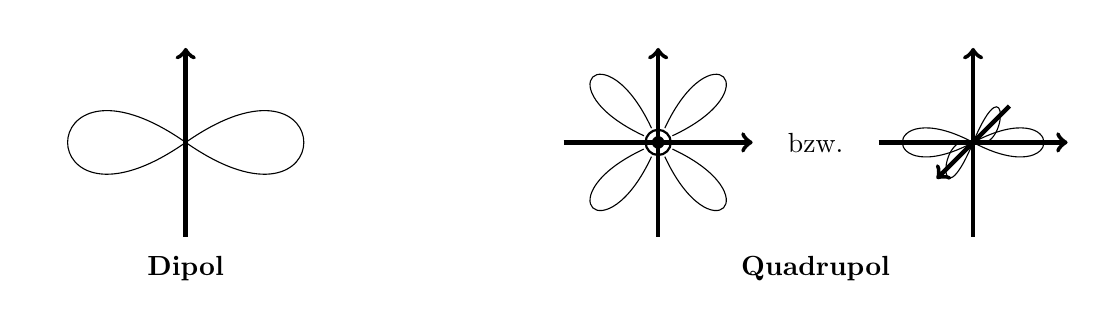
\begin{tikzpicture}[scale=.8]
		\draw [ultra thick,->] (0,-1.5) -- (0,1.5);
		\draw (0,0) .. controls (2.5,1.75) and (2.5,-1.75) .. (0,0);
		\draw (0,0) .. controls (-2.5,1.75) and (-2.5,-1.75) .. (0,0);
		\draw (0,-2) node{\textbf{Dipol}};

		\draw [ultra thick,->] (7.5,-1.5) -- (7.5,1.5);
		\draw [ultra thick,->] (6,0) -- (9,0);
		\draw [thick] (7.5,0) circle (0.2cm);
		\fill (7.5,0) circle (0.1cm);
		\begin{scope}[shorten <= .2cm, shorten >= .2cm]
			\draw (7.5,0) .. controls +(25:2cm) and +(65:2cm) .. (7.5,0);
			\draw (7.5,0) .. controls +(115:2cm) and +(155:2cm) .. (7.5,0);
			\draw (7.5,0) .. controls +(205:2cm) and +(245:2cm) .. (7.5,0);
			\draw (7.5,0) .. controls +(295:2cm) and +(335:2cm) .. (7.5,0);
		\end{scope}
		\draw (10,-2) node{\textbf{Quadrupol}};
		\draw (10,0) node{bzw.};

		\draw [ultra thick,->] (11,0,0) -- (14,0,0);
		\draw [ultra thick,->] (12.5,-1.5,0) -- (12.5,1.5,0);
		\draw [ultra thick,->] (12.5,0,-1.5) -- (12.5,0,1.5);
		\draw (12.5,0,0) .. controls (14,.8,0) and (14,-.8,0) .. (12.5,0,0);
		\draw (12.5,0,0) .. controls (11,.8,0) and (11,-.8,0) .. (12.5,0,0);
		\draw (12.5,0,0) .. controls (12.5,.8,1.5) and (12.5,-.8,1.5) .. (12.5,0,0);
		\draw (12.5,0,0) .. controls (12.5,.8,-1.5) and (12.5,-.8,-1.5) .. (12.5,0,0);
	\end{tikzpicture}}
\caption{Richtungsabhängigkeit der Felder}
\end{figure}

\section{Strahlung einer bewegten Punktladung}

Wir wollen nun die im letzten Kapitel hergeleiteten Formeln auf das Beispiel einer bewegten Punktladung anwenden. Es gilt für die retardierten Potentiale:

\begin{equation*}
\begin{pmatrix}
\varphi\\
\vec{A}
\end{pmatrix}
\left(\vec{r},t\right) \ = \ \begin{pmatrix}
\frac{1}{\epsilon_0}\\
\mu_0
\end{pmatrix}
\ \Int{}{}{V'}\frac{1}{4\pi|\vec{r}-\vec{r}'|} \ \begin{pmatrix}
\rho\\
\vec{j}
\end{pmatrix}
\left(\vec{r}', t \ - \ \frac{|\vec{r}-\vec{r}'|}{c}\right)
\end{equation*}

Für den Spezialfall einer Punktladung auf einer Bahn $\vec{R}(t)$ gilt:

\begin{align*}
\rho(\vec{r},t)  \ &= \ Q \ \delta\left(\vec{r}-\vec{R}(t)\right)\\
\vec{j}(\vec{r},t)  \ &= \ Q \ \vec{R}(t) \ \delta\left(\vec{r}-\vec{R}(t)\right) 
\end{align*}

Einsetzen ergibt:

\begin{align*}
\varphi(\vec{r},t)  \ &= \ \frac{Q}{4\pi\epsilon_0} \ \int\d V'\d t' \frac{\delta(\vec{r}-\vec{R}(t'))}{|\vec{r}-\vec{r}'|} \ \delta\left(t'-t + \frac{|\vec{r}-\vec{r}'|}{c}\right) \\ 
&= \ \frac{Q}{4\pi\epsilon_0}\Int{}{}{t'} \ \frac{1}{|\vec{r}-\vec{R}(t')|} \ \delta \Bigg(t'\underbrace{-t+\frac{|\vec{r}-\vec{R}(t')|}{c}}_{=: -t_0}\Bigg)
\end{align*}

\newpage
\ \\
\ \\
\begin{wrapfigure}[]{c}[0cm]{0cm}
	\raisebox{-.5cm}[\dimexpr\height-1\baselineskip\relax]{
		\colorbox{hgrey}{
			\begin{tikzpicture}[scale=.7]
				\draw [ultra thick,->] (0,0)--(6,0);
				\draw [ultra thick,->] (0,0)--(0,4);
				\fill (5,2) circle(0.1cm) node[right]{Beobachter};
				\draw (5,0.2)--(5,-0.2) node[below]{$t$};
				\draw (0.2,2)--(-0.2,2) node[left]{x};
				\draw (1,0.3)--(5,2);
				\draw (1,3.7)--(5,2);
				\fill [red] (2.4,0.9) circle(0.1cm);
				\draw (0.6,0.75) node[red]{$\vec{R}(t)$};
				\draw [very thick, red] (0.6,1.15) to[out=30, in=140] (2.4,0.9);
				\draw [very thick, ->, red] (2.4,0.9) to[out=320, in=200] (4,0.8) node[right]{Quelle};
				\draw (2.4,0.2)--(2.4,-0.2) node[below]{$t_0$};
				\draw [color=hgrey] (0,4.21) node{a};
			\end{tikzpicture}
		}
	}
	\caption{Bewegte Punktladung}
\end{wrapfigure}

Dies kann man sich mithilfe eines Lichtkegels wie in Abb. 8.2 veranschaulichen.\\
Um die Rechnung weiterzuführen benötigt man:

\begin{equation*}
\delta(f(x))  \ = \  \sum_i \ \frac{\delta(x-x_i)}{\hspace{.65cm}\left|\pdiff{f}{x}\right|_{x=x_i}}
\end{equation*}

wobei die $x_i$ die Nullstellen von $f$ sind.\\
Somit gilt für das Potential:

\begin{equation*}
\varphi(\vec{r},t)  \ = \ \frac{Q}{4\pi\epsilon_0}\cdot \frac{1}{|\vec{r}-\vec{R}(t_0)|} \cdot \left(1\ - \ \frac{\dot{\vec{R}}(t_0) \cdot (\vec{r}-\vec{R}(t_0))}{c \ |\vec{r}-\vec{R}(t_0)|}\right)^{-1}
\end{equation*}\\

Setzen wir nun für den Ausdruck $\vec{r}-\vec{R}$ die Abkürzung $\vec{r}''$ und für $\dot{\vec{R}}$ den Ausdruck $\vec{V}$ ein, erhalten wir die sogenannten \textbf{Liénard-Wiechert-Potentiale}:

\begin{empheq}[box=\highlightbox]{align*}
\varphi(\vec{r},t)  \ &= \ \frac{Q^{\vphantom{\big|}}}{4\pi\epsilon_0} \ \left[\frac{1}{|\vec{r}-\vec{R}| \ - \ \frac{\dot{\vec{R}}}{c} (\vec{r}-\vec{R})}\right]_{\text{ret}}  \ = \ \frac{Q}{4\pi\epsilon_0} \ \left(\frac{1}{r'' \ - \ \frac{ \vec{V}\cdot \vec{r}''}{c}}\right)_{\text{ret}}\\
\ \\
\vec{A}(\vec{r},t) \ &= \ \frac{\mu_0 \ Q}{4\pi} \ \left[\frac{\dot{\vec{R}}}{|\vec{r}-\vec{R}| \ - \ \frac{\dot{\vec{R}}}{c}(\vec{r}-\vec{R})}\right]_{\text{ret}}  \ = \  \frac{\mu_0 \ Q}{4\pi} \ \left(\frac{\vec{V}}{r'' \ - \ \frac{\vec{V}\cdot\vec{r}''}{c}}\right)_{\text{ret}} 
\end{empheq}	

\newpage
\section{Strahlungsbremsung}

Wir wollen in diesem Kapitel eine Punktladung auf einer Bahn 
$\vec{R}(t)$ im nichtrelativistischen Falle betrachten. Dafür berechnen wir zunächst alle benötigten Größen:

\begin{align*}
\rho  \ &= \ Q \delta(\vec{r}-\vec{R}(t))\\
\vec{j}  \ &= \ Q \  \dot{\vec{R}} \ \delta(\vec{r}-\vec{R}(t))\\
\vec{p} \ &= \ \Int{}{}{V}r\rho  \ = \  Q \ \vec{R}(t)\\
\vec{m}  \ &= \ \frac{1}{2} \Int{}{}{V} \vec{r}\times\vec{j}  \ = \ \frac{1}{2}\Int{}{}{V}\vec{r}\times\dot{\vec{R}}\ Q \ \delta(\vec{r}-\vec{R}(t)) \ = \ \frac{Q}{2} \vec{R}\times\dot{\vec{R}}\\
\dot{\tens{D}}'  \ &= \ 3 \Int{}{}{V} \left(\vec{r}\circ\vec{j} \ + \ \vec{j}\circ\vec{r}\right)  \ = \ 3Q \ \left(\vec{R}\circ\dot{\vec{R}} \ + \ \dot{\vec{R}}\circ\vec{R}\right)
\end{align*}

Wie man leicht erkennt hat eine \underline{bewegte} Punktladung auch Multipolmomente. Nun nutzen wir die Dipolnäherung aus Kapitel 8.4 für die abgestrahlte Leistung:

\begin{equation*}
N  \ = \  \frac{\mu_0}{6\pi \ c} \ddot{\vec{p}}^2  \ = \  \underbrace{\frac{\mu_0 \ Q^2}{6\pi \ c}}_{:=\alpha} \ \dot{\vec{v}}^2 \qquad \left(\text{Gültig für } \frac{v}{c}\ll 1\right)
\end{equation*}

Für $\dot{\vec{v}}\neq 0$ verliert das Teilchen also Bewegungsenergie in Form von abgestrahlter elektromagnetischer Leistung. Es wirkt also eine Bremskraft:

\begin{align*}
\Delta W_{\text{elm}}  \ = \ \Int{}{}{t} N  \ &= \ - \Delta W_{\text{mech}}  \ = \  - \Int{}{}{t} \vec{F}_S\cdot\vec{v}\\
\alpha \Int{}{}{t}\dot{\vec{v}}^2  \ &= \ - \Int{}{}{t}\vec{v}\cdot\vec{F}_s \ \overset{\text{part. Int.}}{=} \ - \alpha\Int{}{}{t}\ddot{\vec{v}}\vec{v} \ + \ \left.\alpha\vec{v}\dot{\vec{v}}\right|^{t_2}_{t_1} 
\end{align*}

Der Randterm verschwindet dabei für oszillierende Bewegungen, sodass man die Bremskraft $\vec{F}_S$ explizit ausrechnen kann mit:

\begin{empheq}[box=\highlightbox]{equation*}
\vec{F}_S \ = \ \alpha \ddot{\vec{v}}  \ = \ \frac{Q^2\vphantom{\big|}}{6\pi\epsilon_0 \ c^3\vphantom{\big|}} \dddot{\vec{R}}
\end{empheq}

Diese Formel ist allerdings nur anwendbar, wenn $\vec{F}_S$ eine kleine Korrektur ist.